\subsection{High Level Message Sequence Chart}
	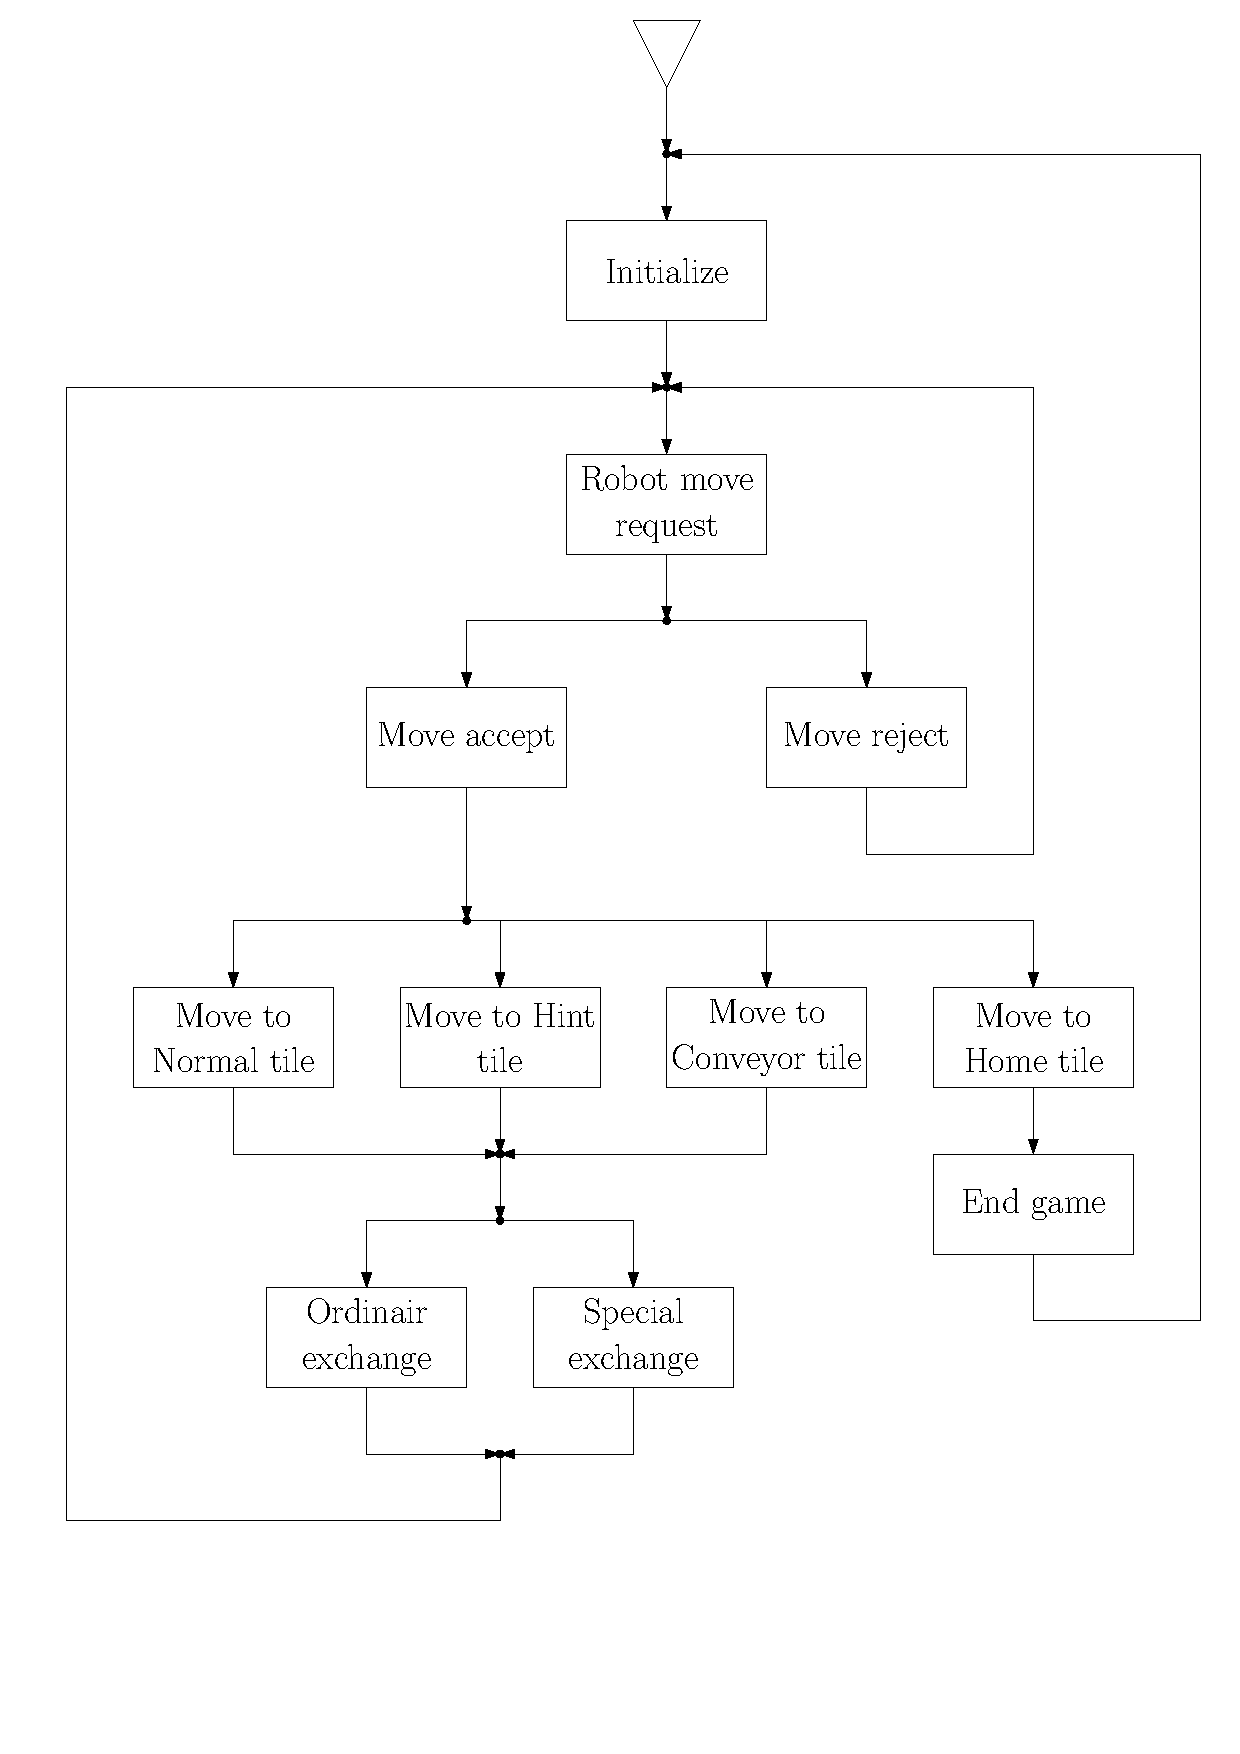
\includegraphics[width=\linewidth]{MSC-files/HMSC.pdf}
	
\subsection{Message Sequence Charts}
	\subsubsection{Robot move - OK}
	\begin{msc}
		msc
		{

		a [label="Robot type A"],
		b [label="Robot type B"],
		c [label="Controller"],
		d [label="Board"];

		a box a [label=""],
		b box b [label=""],
		c box c [label=""],
		d box d [label=""];

		|||;

		a -> c [label="Move request"];
		c => d [label="Move OK?"];
		d >> c [label="OK"];
		c => d [label="Make move"];
		d box d [label="Save location of robot"];
		d >> c [label="OK"];
		c -> a [label="OK"];

		|||;

		---;

		|||;

		b -> c [label="Move request"];
		c => d [label="Move OK?"];
		d >> c [label="OK"];
		c => d [label="Make move"];
		d box d [label="Save location of robot"];
		d >> c [label="OK"];
		c -> b [label="OK"];

		|||;

		a box a [label="", textbgcolor="black"],
		b box b [label="", textbgcolor="black"],
		c box c [label="", textbgcolor="black"],
		d box d [label="", textbgcolor="black"];

		}
	\end{msc}
	
	\subsubsection{Robot move - Not OK}
	\begin{msc}
		msc
{

a [label="Robot type A"],
b [label="Robot type B"],
c [label="Controller"],
d [label="Board"];

a box a [label=""],
b box b [label=""],
c box c [label=""],
d box d [label=""];

|||;

a -> c [label="Move request"];
c => d [label="Move OK?"];
d >> c [label="NOK"];
c -> a [label="NOK"];

|||;

---;

|||;

b -> c [label="Move request"];
c => d [label="Move OK?"];
d >> c [label="NOK"];
c -> b [label="NOK"];

|||;

a box a [label="", textbgcolor="black"],
b box b [label="", textbgcolor="black"],
c box c [label="", textbgcolor="black"],
d box d [label="", textbgcolor="black"];

}

	\end{msc}
	
	\subsubsection{Robot move - Hint tile}
	\begin{msc}
		msc
{

a [label="Robot type A"],
b [label="Robot type B"],
c [label="Controller"],
d [label="Board"];

a box a [label=""],
b box b [label=""],
c box c [label=""],
d box d [label=""];

|||;

a -> c [label="Move request"];
c => d [label="Move OK?"];
d >> c [label="OK"];
c => d [label="Make move"];
d >> c [label="Hinttile"];
c => d [label="Get Hint"];
d rbox d [label="Generate hint"];
d >> c [label="Hint"];
c -> a [label="Hint"];

|||;

---;

|||;

b -> c [label="Move request"];
c => d [label="Move OK?"];
d >> c [label="OK"];
c => d [label="Make move"];
d >> c [label="Hinttile"];
c => d [label="Get Hint"];
d rbox d [label="Generate hint"];
d >> c [label="Hint"];
c -> b [label="Hint"];

|||;

a box a [label="", textbgcolor="black"],
b box b [label="", textbgcolor="black"],
c box c [label="", textbgcolor="black"],
d box d [label="", textbgcolor="black"];

}
	\end{msc}
	
	\subsubsection{Robot move - Conveyor Belt}
	\begin{msc}
		msc
{

a [label="Robot type A"],
b [label="Robot type B"],
c [label="Controller"],
d [label="Board"];

a box a [label=""],
b box b [label=""],
c box c [label=""],
d box d [label=""];

|||;

a -> c [label="Move request"];
c => d [label="Move OK?"];
d >> c [label="OK"];
c => d [label="Make move"];
d >> c [label="OK"];
c => d [label="Make move"];
d >> c [label="Conveyer belt"];
c -> a [label="Conveyer belt"];

|||;

---;

|||;

a -> c [label="Move request"];
c => d [label="Move OK?"];
d >> c [label="OK"];
c => d [label="Make move"];
d >> c [label="OK"];
c => d [label="Make move"];
d >> c [label="Conveyer belt"];
c -> a [label="Conveyer belt"];

|||;

a box a [label="", textbgcolor="black"],
b box b [label="", textbgcolor="black"],
c box c [label="", textbgcolor="black"],
d box d [label="", textbgcolor="black"];

}
	\end{msc}
	
	\subsubsection{Robot move - Home tile}
	\begin{msc}
		msc
{

a [label="Robot type A"],
b [label="Robot type B"],
c [label="Controller"],
d [label="Board"];

a box a [label=""],
b box b [label=""],
c box c [label=""],
d box d [label=""];

|||;

a -> c [label="Move request"];
c => d [label="Move OK?"];
d >> c [label="OK"];
c => d [label="Make move"];
d rbox d [label="Save location of robot"];
d rbox d [label="Save which robot wins"];
d >> c [label="WIN"];
c -> a [label="WIN"];
d rbox d [label="Destroy rest"];

|||;

---;

|||;

b -> c [label="Move request"];
c => d [label="Move OK?"];
d >> c [label="OK"];
c => d [label="Make move"];
d rbox d [label="Save location of robot"];
d rbox d [label="Save which robot wins"];
d >> c [label="WIN"];
c -> b [label="WIN"];
d rbox d [label="Destroy rest"];

|||;

a box a [label="", textbgcolor="black"],
b box b [label="", textbgcolor="black"],
c box c [label="", textbgcolor="black"],
d box d [label="", textbgcolor="black"];

}

	\end{msc}
	
	\subsubsection{Tiles exchange}
	\begin{msc}
		msc
{

b [label="Board"],
c [label="Controller"],
p1 [label="Player 1"],
p2 [label="Player 2"];

b box b [label=""],
c box c [label=""],
p1 box p1 [label=""],
p2 box p2 [label=""];
|||;
c=>b [label="Get two valid tiles"];
b>>c [label="two valid tiles"];
c=>b [label="exchange tiles"];
b rbox b [label="exchange two tiles"];
b->c [label="tiles exchanged"];
...;
c->p1 [label="board changed"];
c->p2 [label="board changed"];
...;

|||;

b box b [label="",textbgcolor="black"],
c box c [label="",textbgcolor="black"],
p1 box p1 [label="",textbgcolor="black"],
p2 box p2 [label="",textbgcolor="black"];

}

	\end{msc}
	
	\subsubsection{Tiles exchange special}
	\begin{msc}
		msc
{

b [label=""],
c [label=""],
p1 [label=""],
p2 [label=""];

b box b [label="Board"],
c box c [label="Controller"],
p1 box p1 [label="Robot player 1"],
p2 box p2 [label="Robot player 2"];
|||;
c=>b [label="Get two valid tiles"];
b>>c [label="two valid tiles"];
c=>b [label="exchange tiles"];
b rbox b [label="exchange two tiles"];
b rbox b [label="rotate robot player 1 and conveyer belt"];
b->c [label="tiles exchanged"];
...;
c->p1 [label="board changed"];
c->p1 [label="robot rotated"];
c->p2 [label="board changed"];
...;

}

	\end{msc}
	